\section{DensePose - Related work}

\noindent 
\textbf{DensePose task.} DensePose-COCO dataset contains a large set of images of people collected ``in the wild'' together with different annotations: (i) bounding boxes, (ii) foreground-background masks, (iii) dense correspondences --- points $p \in S$ of a reference 3D model $S\in\mathbb{R}^3$ of the object associated with triplets $(c, u, v) \in\{1, \ldots, C\} \times[0,1]^{2}$, where $c$ indicates which one of $C$ body parts contains the pixel and $(u,v)$ represents the corresponding location (UV coordinates) in the chart of the part \cite{smpl}.
The DensePose task is then to predict such triplets $(c, u, v)$ for each foreground pixel and every person in the image.
\newline

\noindent \textbf{DensePose R-CNN.} The baseline dense pose prediction model, and all the subsequent works \cite{parsing, uncertainty, monkeys} follow the architecture design of Mask R-CNN \cite{maskrcnn}.

The model is a two-stage: first, it generates class-independent region proposals (boxes), then classifies and refines them using the box/class head. Finally, the DensePose head predicts the body part and UV coordinates for each pixel inside the box. Particularly, the model consists of many different blocks (see Fig.~\ref{fig:scheme}):
\begin{itemize}
    \item \textit{Backbone} to extract features from the image,
    \item \textit{Neck} to integrate features from different feature levels of the backbone to effectively perform multi-scale detection,
    \item \textit{Region proposal network (RPN)} to propose a sparse set of box candidates potentially containing objects,
    \item \textit{Heads} take the features pooled from the bounding box on the corresponding feature level, where the detection occurred, and produce output. The first head is a box/class head, which finally predicts whether the object is present in the box and refines the box coordinates. The second head is the DensePose head that predicts either the pixel belongs to the background or assigns it to one of the 24 DensePose charts, and regresses UV coordinates to each foreground pixel inside the bounding box.
\end{itemize}

\noindent \textbf{Model architecture optimisation.}
In recent years the neural architecture search (NAS) techniques gained popularity \cite{automl}. The main aim of NAS is to find the optimal architecture under specific hardware requirements. Usually, these techniques are applied in simple setups, e.g., classification networks, or in the case of two-stage object detection models, NAS is usually applied to individual parts of the model \cite{nasfpn}. In this paper, instead of creating one more design for a particular part of the model, we try to test different existing approaches and see what works best for the DensePose estimation task. Particularly, we evaluate several backbones that were a result of NAS optimization and try to test them out with other components.

\begin{figure}[!hbtp]
\centering
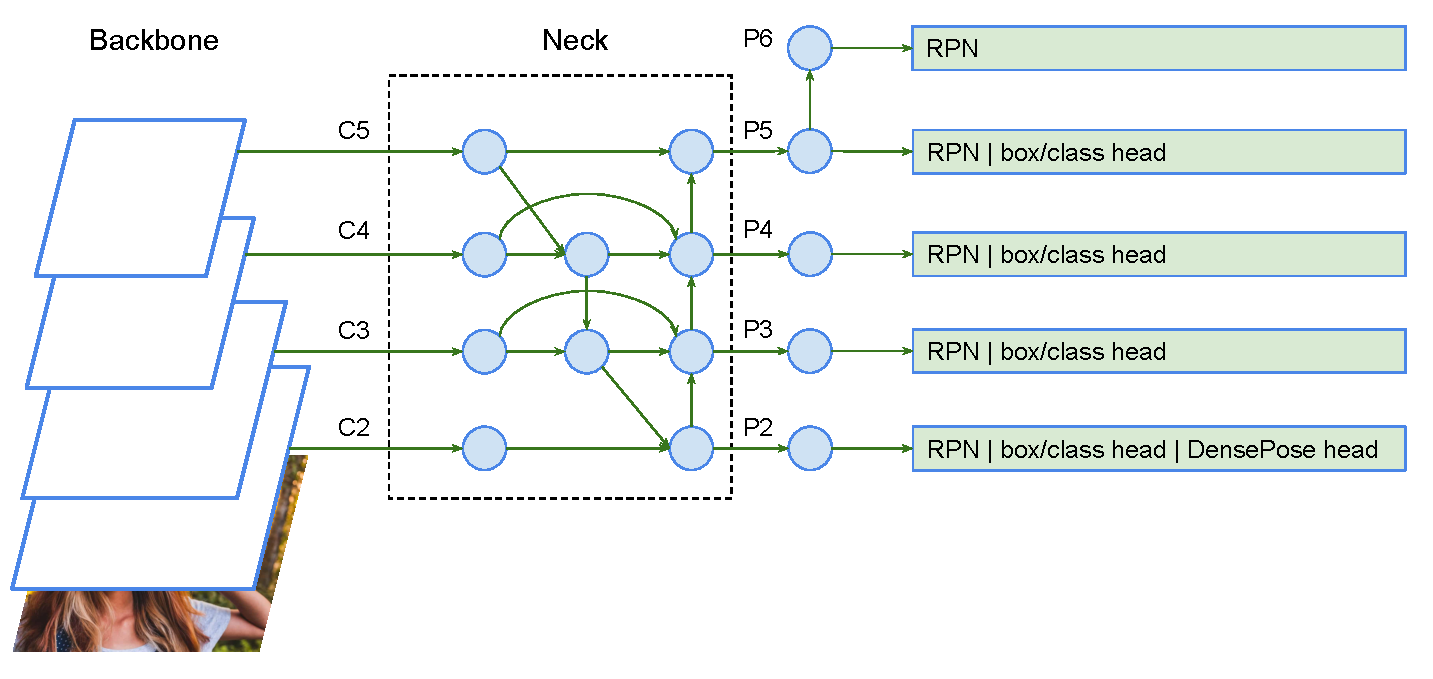
\includegraphics[width=0.4\textwidth]{Figures/densepose/scheme.pdf}
\caption{The high level structure of the Mobile Parsing R-CNN model. $C_i$, $P_i$ represent feature levels with a resolution of $1/2^i$ of the input image. $P_6$ is obtained via stride-2 pooling on $P_5$.}
\label{fig:scheme}
\end{figure}